\documentclass[main]{subfiles}

% \setlength{\tabcolsep}{10pt} % Default value: 6pt
% \renewcommand{\arraystretch}{1.5} % Default value: 1

\begin{document}
\newpage
\section{Learning As Bayesian Inference}

\subsection{Motivation}
The main idea of this chapter is to study how to incorporate model uncertainty relying on Bayesian modelling. First, let us discuss briefly why model uncertainty is a great quantity to possess.

\subsubsection{Why uncertainty matters?}
    \paragraph{On the biological side:} we, humans, incorporate uncertainty in our decisions. We live in an environment where we need to act fast based on noisy, ambiguous and sparse sensory information. Therefore, decisions are usually made under substantial uncertainty. In fact a Bayesian brain hypothesis suggests that the brain follows a Bayesian probabilistic framework to make optimal decisions in presence of uncertainty \footnote{Knill DC, Pouget A (2004) The bayesian brain: the role of uncertainty in neural coding and computation. TRENDS in Neurosciences 27(12):712–719}.
    
    For instance, our visual systems are subject to uncertainty due to noisy inputs \footnote{Uncertainty in visual processes predicts geometrical optical illusions}
    \begin{figure}[H]
    	\centering
    	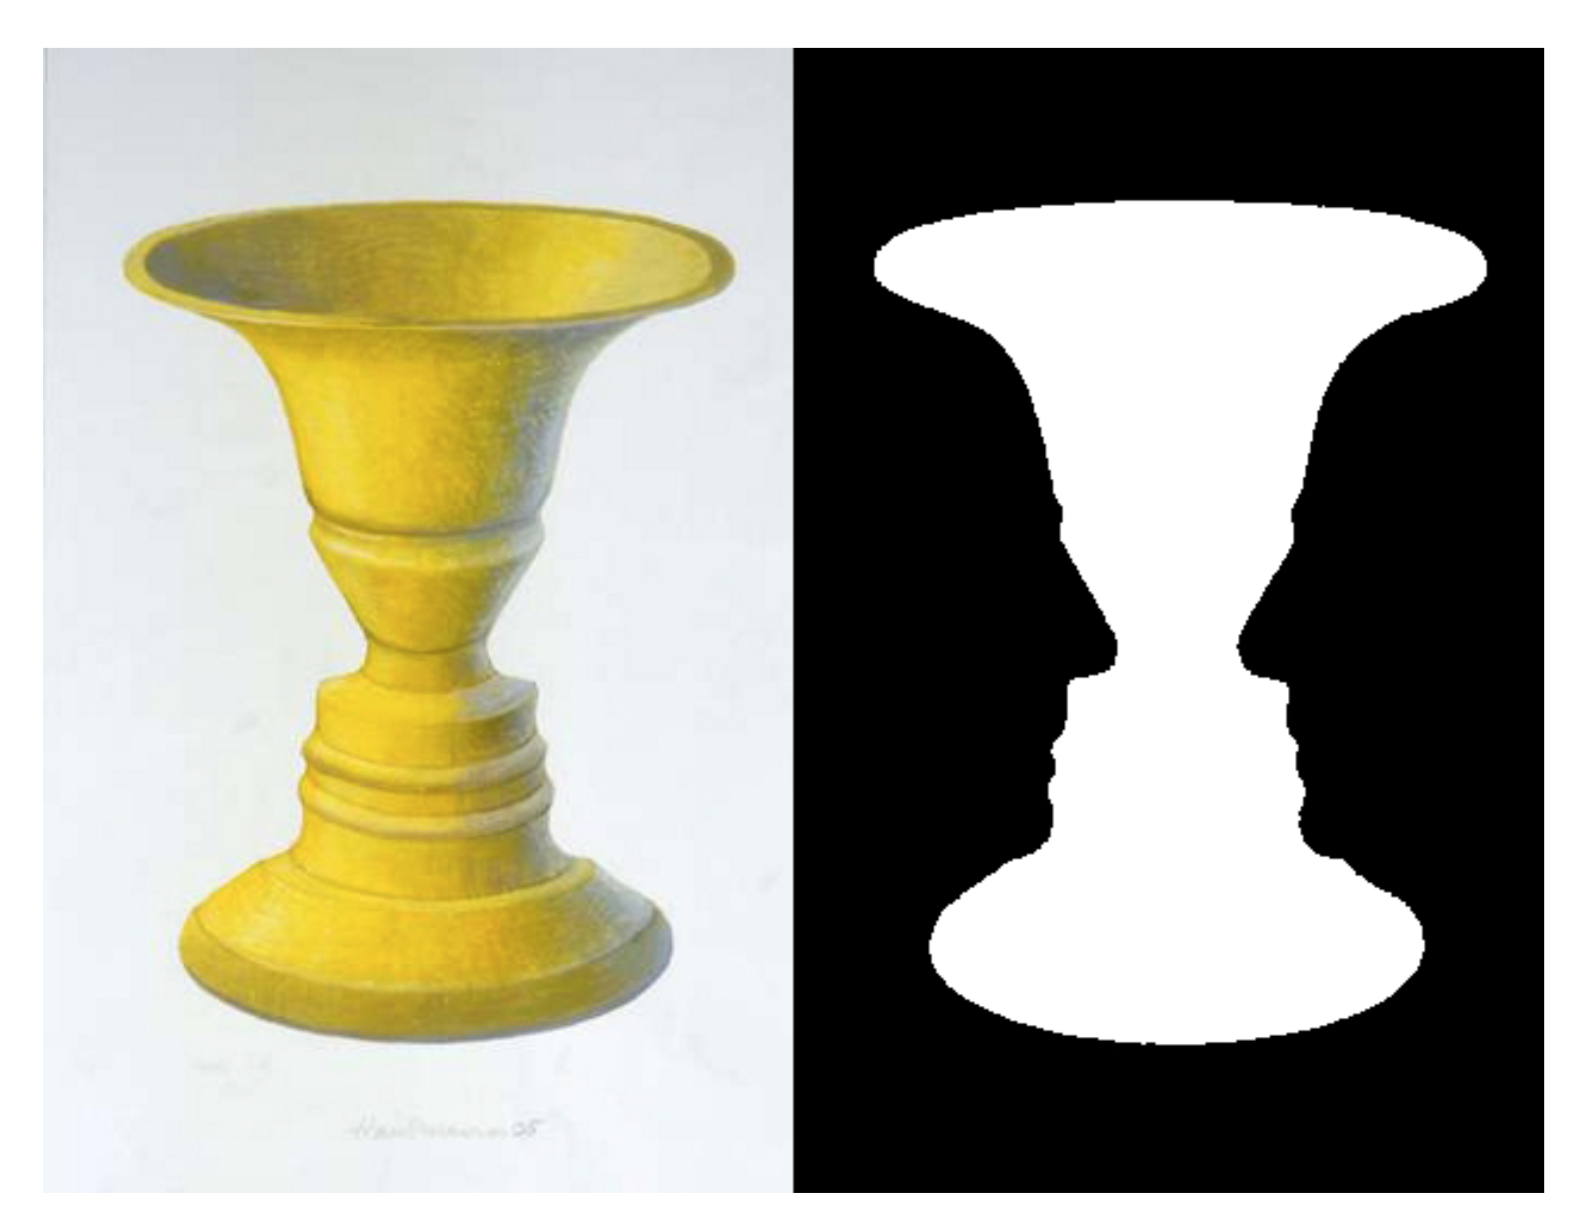
\includegraphics[width=0.5\linewidth]{05_LearningAsBayesianInference/figures/rubinvase.png}
    	\caption{Rubin's vase. Illustration of competing plausible explanations of the world. What should we see? a vase (on a black background) or two faces (on a white background)?}
    	\label{fig:visual_illusion}
    \end{figure}
    
    \noindent
    More formally, uncertainty is incorporated in every stage of neural computation because:
    \begin{itemize}
        \item[--] Real sensors are noisy (e.g., low light vision)
        \item[--] Real systems have finite computational resources
        \item[--] Data is finite (e.g., we work with finite N in our learning problem)
    \end{itemize}
    
    \paragraph{Applications side:} for building systems that make critical decisions, it becomes increasingly important to incorporate the model uncertainty information. For example, systems for automated diagnosis, autonomous driving or computers taking control over systems that can destabilize entire economic markets.\footnote{Yarin Gal."Uncertainty in deep learning",PhD thesis, University of Cambridge, 2016.}

\subsection{Learning as an Optimization Problem}
\subsubsection{Recap: Learning from Data}
Till now, we have talked about the standard view of learning. In this view, the recipe to learn from data is as follows:

\begin{quote}
    Consider a supervised learning problem, we are given a dataset of N training examples with their corresponding targets $t$ $D = {(x^{(n)}, t^{(n)})}$ and a neural network model $f_{NN}$. Our goal is to find the 
\begin{enumerate}
    \item Define a global loss function, for instance a squared loss
        \begin{equation}
            L(w) = \frac{1}{2} \sum_{n=1}^{N} \parallel t^{(n)} - f_{NN}(x^{(n)},w) \parallel
        \end{equation}
    \item Systematically update the model parameters (i.e weights) to minimize L relying on the gradients of L. In DL, the common method is backprop.
    
        \begin{equation}
            \Delta w = -\eta \bigtriangledown_w L(w)
        \end{equation}
    
\end{enumerate}
\end{quote}

\paragraph{Why does it work?}
\hl{...}
\paragraph{Credit assignment:} "The concept of credit assignment refers to the problem of determining how much ‘credit’ or ‘blame’ a given neuron or synapse should get for a given outcome." \footnote{Richards, Lillicrap, Therien* et al. A deep learning framework for neuroscience, 2019.}
\noindent It can be formulated as an optimization problem. However, we must distinguish between pure (traditional) optimization and the optimization used for training of deep models.

\subsubsection{How learning differs from pure optimization?}
In ML scenarios, we try to optimize a performance metric indirectly via a loss function. In other words, initially, we care about a performance measure, $P$, with respect to the test set. However, since optimizing $P$ directly is often intractable, we tend to reduce a different cost function $J(\theta)$ with the hope that this will improve $P$ as well). In contrast, in traditional optimization problems $J(\theta)$ is a goal in itself.\footnote{Chapter 8 Optimization for training Deep Models.Deep Learning}
    

\subsection{Neural Network Models of the brain}
\hl{...}

\subsection{Interlude on Bayesian Modelling}
Bayesian probability theory provides us with the tools to incorporate model uncertainty estimates in NN.
   
\noindent Following Bayesian approach, the idea is to start with an initial estimate of how the parameters are distributed and update our belief once data is observed. 

\noindent
\textbf{Note that: under this view the weights not single-valued (point estimates) but are random variables coming from a probability density function (pdf). In other words, weights are represented by probability distributions.}

\subsubsection{Model Definition}
In Bayesian modelling, we need to define 2 components:
        \begin{enumerate}
            \item A \textbf{prior distribution} over the parameters space \textbf{$p(w)$} which represents our prior belief on to which parameters are \textit{likely} to have generated the data \textbf{before} we have seen the dataset. 
            
            \item A probabilistic model \textbf{$p(t|x,w)$}, \textbf{the likelihood distribution or function}, by which the inputs generate the output given some network parameter setting.
        \end{enumerate}
        
Once some data is observed, the weight distribution is updated to get the \textit{posterior distribution} $p(w|D)$ of the weights given the data. Using Bayes rule, we can compute the posterior. 

\paragraph{Bayes Rule:}
    \begin{equation}
    \boxed{
        posterior = \frac{prior . likelihood}{evidence }
        }
    \end{equation}

\paragraph{Posterior distribution of w:}
\begin{equation}
    \boxed{
    p(w|D) = \frac{p(t|x,w). p(w)}{\int_\Omega p(t|x,w). p(w) dw}
    }
    \label{eq:posterior distribution}
\end{equation}

\begin{itemize}
    \item[--] $\Omega$ is the weight space 
    \item[--] The denominator in eq.\ref{eq:posterior distribution} is \textbf{the model evidence} also called \textbf{the normalizing factor}. It represents $p(t|x)$ which is computed by marginalizing the likelihood over w (integrating out over the entire parameter space). This integration is usually hard to carry out analytically for complex models. In such cases approximation is needed.
\end{itemize}

\subsection{Recovering the optimization view of learning}
In this section, we will try to connect between the two views to learning: the standard and probabilistic view. Both boil down to solving an optimization problem.

% \paragraph{Recap}
% \begin{itemize}
%     \item We are trying to
% \end{itemize}
\paragraph{Assumptions}
\begin{itemize}
    \item[--] In regression tasks, we assume a Gaussian model, i.e.
    \begin{equation}
        (t^{(n)}| x^{(n)},w) \sim N(t^{(n)}; f_{NN}(x^{(n)},w), \sigma^2 I)
    \end{equation}
    where $f_{NN}(x^{(n)},w)$ and $\sigma^2 I$ are the mean and variance of the normal distribution. We can therefore write the likelihood function as the product of individual samples.
    
    \begin{equation}
        p(t^{(n)}| x^{(n)},w) = \Pi_{n=1}^{N} N(t^{(n)}; f_{NN}(x^{(n)},w), \sigma^2 I)
    \end{equation}
    \item[--] Weights are independent and identically distributed (iid) and follow a normal distribution as well. Assume there are K weights (i.e dim
    \begin{equation}
        p(w) = \Pi_{k=1}^{K} N(w_k; 0, \sigma^2_w)
    \end{equation}
\end{itemize}

\paragraph{Interlude I: Point estimate for the posterior}
Using the fact that the likelihood and the priors are both normal distributions we can easily compute a single point estimate (i.e a single value that serves as a "best guess" for the weights matrix). This point estimate can be the mode of the distribution computed as
\begin{equation}
    w^* = \argmax_w p(\bm{w}|D)
\end{equation}

\noindent That is the value that maximizes the posterior $p(\bm{w}|D)$, also called \textbf{maximum a posteriori estimate} of the weights. 
Using some analytical manipulations, we can show that
\begin{equation}
    \hl{...}
\end{equation}

\noindent However, as we will see later, using the mode of the posterior doesn't help much. In fact, summarizing the posterior with a single point estimate again leads to the same problem we are trying to avoid, which is a single "best" value for the weights, i.e a single line separating the data (in the context of stochastic binary classification). 
\begin{figure}[H]
    	\centering
    	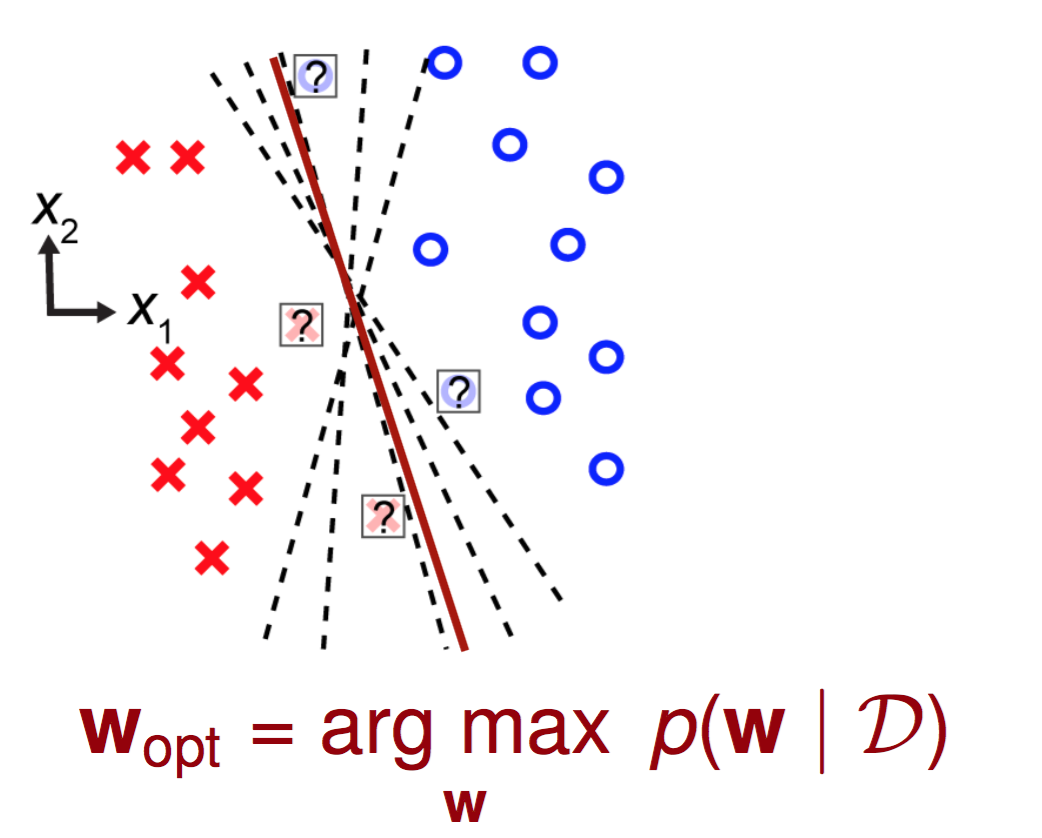
\includegraphics[width=0.6\linewidth]{05_LearningAsBayesianInference/figures/posteriormode_classifier.png}
    	\caption{Maximum a posteriori estimate of the weights yields single line classifying the data}
    	\label{fig:posterior_mode_classifier}
    \end{figure}

\paragraph{Interlude II: Bayesian Predictions}
In order to make predictions on new unseen data, we would have to predict $t^{(N+1)}$ for the new data $\bm{x}^{(N+1)}$.\\

\noindent In the Bayesian approach, this can be done using \textbf{model averaging}. The idea here is that instead of relying on a single model to make the prediction, we average the predictions from all possible models or \textit{model ensemble}. Therefore, the probability that the new $\bm{x}^{(N+1)}$ belongs to label $t^{(N+1)} = 1$ is given by

\begin{equation}
    \begin{split}
        P(t^{(N+1)} = 1 |\bm{x}^{(N+1)}, D) &= \EX_{w \sim p(w|D)}[y(\bm{x}^{(N+1)},w)] \\
    &=\int_{\Omega} y(\bm{x}^{(N+1)},w) p(\bm{w}|D) dw
    \end{split}
    \label{eq:prediction}
\end{equation}

\noindent Once again, we need the full posterior over the weights to make the predictions. But we might ask \textbf{why not use the mode of the posterior to make the predictions?}
\noindent
Another way of phrasing the question: \textbf{why not use the "plug-in" solution where we collapse $p(\bm{w}|D)$ into its mode $\delta(\bm{w}-\bm{w}_{opt})$ (the one computed on \textit{Interlude I}?}

\begin{itemize}
    \item[--] By construction, using the mode we ignore any uncertainty in parameter choice. We only consider the optimal case
    \begin{figure}[H]
    	\centering
    	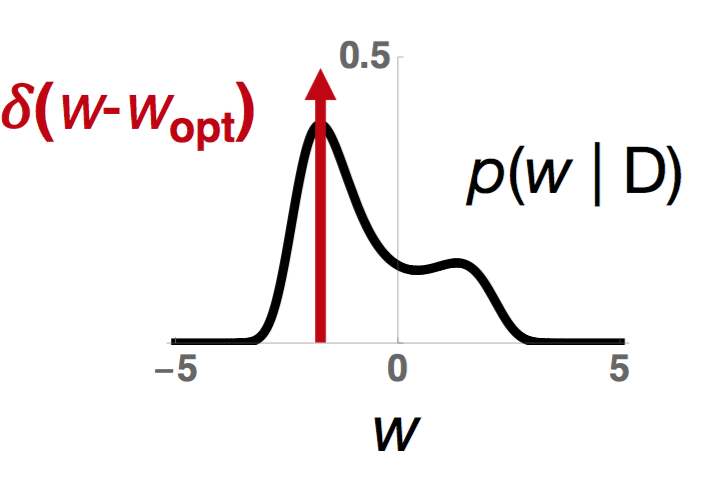
\includegraphics[width=0.6\linewidth]{05_LearningAsBayesianInference/figures/posteriormode_delta.png}
    	\caption{Posterior mode is the optimal case scenario for $p(\bm{w}|D)$}
    	\label{fig:posterior_mode_delta}
    \end{figure}

    \item[--] Therefore, we are bound to make overconfident predictions
    \item[--] We cannot compare different models 
\end{itemize}

\noindent Now that we are convinced that we need the full posterior, we are faced with a problem.
\paragraph{Problem:}As mentioned earlier  the denominator in eq. \ref{eq:posterior distribution} is often intractable. 
\begin{equation*}
    p(\bm{w}|D) = \frac{p(t|\bm{x},\bm{w}).p(\bm{w})}{\int_\Omega p(t|\bm{x},\bm{w}). p(\bm{w}) d\bm{w}}
\end{equation*}
 
\begin{quote}
    \textbf{Solution:} Approximate $p(\bm{w}|D)$ by another, simpler distribution denoted $q(\bm{w})$ from \underline{which we can easily sample} (this would become clearer later)
\end{quote}

\paragraph{Discuss:} Are we still "Bayesian optimal" if we follow this strategy?\\

\hl{...}


\subsubsection{Approximating the posterior $p(w|D)$}
\textbf{Goal:} Find distribution $q(\bm{w})$ that approximates (i.e. is as similar as possible) $p(\bm{w}|D)$. For that, we need to define a measure of distance.\\
\begin{figure}[H]
    	\centering
    	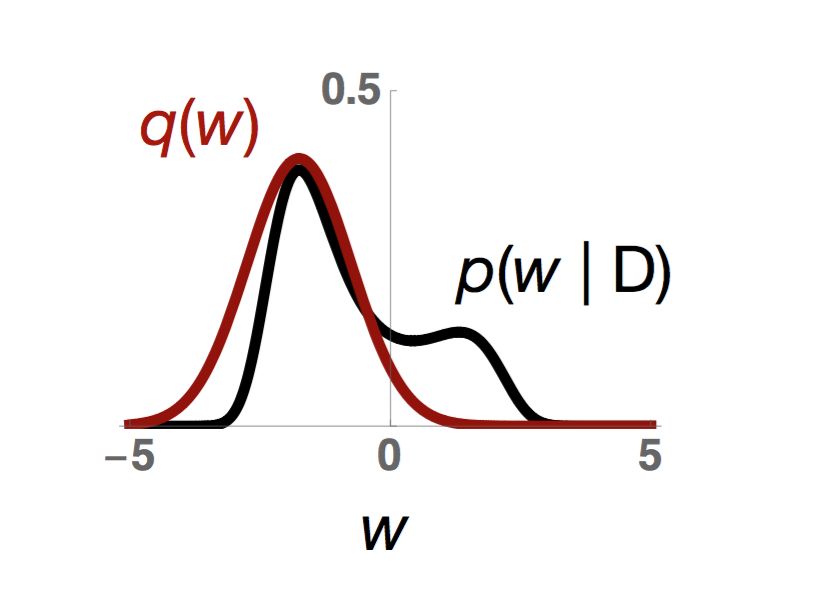
\includegraphics[width=0.6\linewidth]{05_LearningAsBayesianInference/figures/q_posterior.png}
    	\caption{$q(\bm{w})$ is a surrogate distribution \textit{similar} to $p(\bm{w}|D)$}
    	\label{fig:q_posterior}
    \end{figure}
\paragraph{Interim: Kullback-Leibler (KL) Divergence}\\

The Kullback-Leibler divergence between two densities q and p is
defined as

\begin{equation}
    D_{KL}(q(\bm{w})||p(\bm{w}) = \int_\Omega q(\bm{w}) . log \frac{q(\bm{w})}{p(\bm{w}} d\bm{w}
    \label{eq:KL}
\end{equation}

\textbf{Properties of KL divergence}
\begin{itemize}
    \item $D_{KL}$ is not a true measure of distance since in general \\ $D_{KL}(q(\bm{w})||p(\bm{w}) \neq D_{KL}(p(\bm{w})||q(\bm{w})$.\\ It is \textbf{not symmetric} in its arguments.
    \item $D_{KL}$ \textbf{does not obey} the triangle inequality
    \item $D_{KL}(p(\bm{w})||q(\bm{w}) \geq{0}$ (\textbf{Gibb's inequality})
    \item $D_{KL}(p(\bm{w})||q(\bm{w})={0}$ \textbf{if and only if} $q(\bm{w}) = p(\bm{w})$ for almost all $\bm{w}$ (i.e. the two distributions coincide)
\end{itemize}

\subsubsection{Learning as a Variational Inference (VI)}
Consider a simpler weight distribution $q(\bm{w})$ parametrized by $\theta$. The KL divergence \textbf{"from"} the true posterior\textbf{ "to" }q can be written as:
\begin{equation}
    D_{KL}(q(\bm{w}; \theta)||p(\bm{w} |D) = \int_\Omega q(\bm{w};\theta) . log \frac{q(\bm{w};\theta)}{p(\bm{w}|D} d\bm{w}
\end{equation}

\noindent
\textbf{Variational learning} finds the parameters $\theta$ of a distribution on the weights $q(\bm{w};\theta)$ that \textbf{minimises} the KL divergence. However note that we are minimizing over the parameter $\theta$ not the weights


\begin{equation}
\boxed{
    \theta_{opt} = \argmin_\theta D_{KL}(q(\bm{w}; \theta)||p(\bm{w} |D)
    }
    \label{eq:VI_def}
\end{equation}

Using the definition of $D_{KL}$ in eq.\ref{eq:VI_def} and considering that the posterior $p(\bm{w}|D) \propto p(\bm{w}). p(D|\bm{w})$, we can write: \hl{continue derivation from the exercise}
\begin{equation}
    \begin{split}
        \theta_{opt} &= \argmin_\theta \int q(\bm{w};\theta) . log \frac{q(\bm{w};\theta)}{p(\bm{w}|D)} d\bm{w}\\
        &= \argmin_\theta \int q(\bm{w};\theta) . \log \frac{q(\bm{w};\theta)}{p(\bm{w}). p(D|\bm{w})} d\bm{w}\\
        &= \argmin_\theta \int q(\bm{w};\theta). \log \frac{q(\bm{w};\theta)}{p(\bm{w})}  d\bm{w} - \int q(\bm{w};\theta).\log p(D|\bm{w})d\bm{w}\\
        &= \argmin_\theta \EX_{\bm{w} \sim q(\bm{w};\theta)} [-\log p(D|\bm{w})] + D_{KL}(q(\bm{w}; \theta)||p(\bm{w}))\\
        &= \argmin_\theta F(\theta, D)
    \end{split}
    \label{eq:VI_opt}
\end{equation}

\noindent The resulting cost function is known as the \textbf{variational free energy} or \textbf{the expected lower bound} \footnote{Blundell, Cornebise, et al. Weight Uncertainty in Neural Networks. 2015.}. \\It is composed of two terms:
\begin{enumerate}
    \item \underline{Data fitting term}: the expected loss over q
    \item \underline{Prior matching term}: $D_{KL}(q(\bm{w}; \theta)||p(\bm{w}))$. From an information theory viewpoint, this term defines how many nats needed to encode model \hl{explain}
\end{enumerate}

Since we choose $q(\bm{w})$ to be easy to sample from, we can therefore approximate the true mean of the distribution using the sample average.

\begin{equation}
    \EX_{\bm{w} \sim q} [f(\bm{w}] \approx \frac{1}{R} \sum_{r=1}^{r=R} f(\bm{w}^{(r)});
\end{equation}
where R is the number of samples and $\bm{w}^{(r)} \sim q(\bm{w})$\\

\noindent
The optimization of eq.\ref{eq:VI_opt} can be carried out using the gradient. In this case, we compute the derivative
\begin{equation}
    \frac{\partial}{\partial \theta} \EX_{\bm{w} \sim q} [f(\bm{w}] = \frac{\partial}{\partial \theta} \int q(\bm{w};\theta) f(\bm{w}) d\bm{w}
\end{equation}

Note that it would be easier if we swap the derivative and the expectation. 

\subsubsection{Bayes by Backprop (BbB)}
\paragraph{Quick Recap:}
\begin{itemize}
    \item Bayesian inference for neural networks calculates the posterior distribution of the weights given the training data, $p(\bm{w}|D)$.
    \item Remember that all weights in our neural networks are represented by probability distributions over possible values, rather than having a single fixed value as is the norm (see Figure.\ref{fig:BbB_network}).
    \item This distribution answers predictive queries about unseen data by taking expectations.
    \item However, the posterior is untractable and we approximate is using another parametric distribution $q(\bm{w})$
    \item Our goal is to find $\theta$ such that KL-divergence from $p(\bm{w}|D)$ to $q(\bm{w})$ is minimized.
    \item The optimization function $F(\theta, D)$ is composed of two terms: data-independent term, the prior matching and a data-fitting term, which is an expectation over q
    \item Now we are trying to use gradient based technique to solve this optimization problem and would love to swap the expectation and the derivative
        % \item Once again we reached an optimization problem that we hope we can solve using gradient-based techniques.
\end{itemize}

\begin{figure}[H]
    	\centering
    	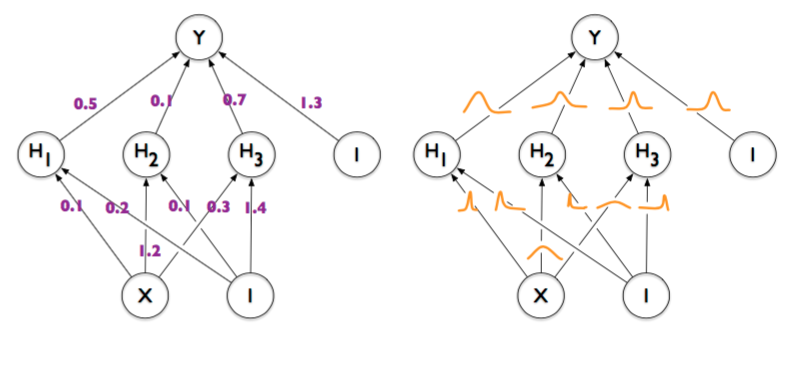
\includegraphics[width=0.9\linewidth]{05_LearningAsBayesianInference/figures/BbB_network.png}
    	\caption{\textbf{Left}: each weight has a fixed value, as provided by classical backpropagation. \textbf{Right}: each weight is assigned a distribution, as provided by Bayes by Backprop.} 
    	\label{fig:BbB_network}
    \end{figure}
    


\noindent Under certain conditions, the expectation of the derivative can be expressed as the derivative of the expectation.

\paragraph{Proposition:} Suppose the weights are independently and modelled by a Gaussian random variables parametrized by the mean, $\mu_k$ and the variance $\sigma^2_k$, i.e.
\begin{equation}
    \begin{split}
        & w_k \sim N(\mu_k,\sigma^2_k)\\
        & \theta_k = (\mu_k,\sigma^2_k)
    \end{split}
\end{equation}

\noindent Now let $w_k  = \mu_k + \sigma_k \epsilon$; where $\epsilon \sim N(0,1)$. Using this reparametrization trick (by introducing $\epsilon$), $\bm{w}$ is no longer the "source of randomness"; $\epsilon$ now is. Therefore, we can propagate the derivative inside the expectation ($\epsilon$ is the random variable)\footnote{\url{https://stats.stackexchange.com/questions/199605/how-does-the-reparameterization-trick-for-vaes-work-and-why-is-it-important}}.

\begin{figure}[H]
    	\centering
    	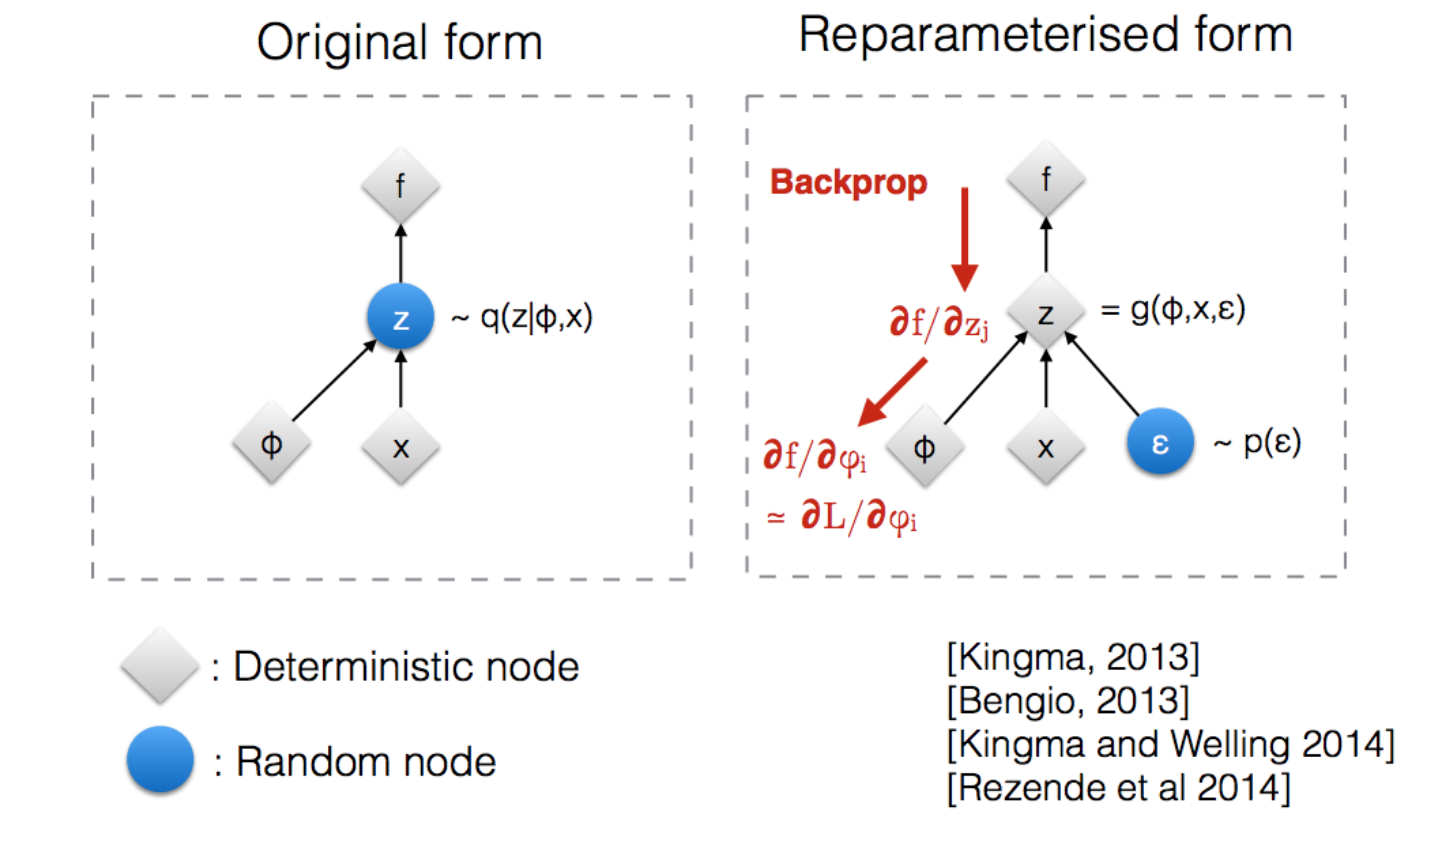
\includegraphics[width=0.9\linewidth]{05_LearningAsBayesianInference/figures/reparametrization.png}
    	\caption{Reparametrization trick intuition. Extracted from..} 
    	\label{fig:reparam_trick}
\end{figure}
    
\begin{equation}
    \begin{split}
        % \frac{\partial}{\partial \theta} \EX_{\bm{w} \sim q} [f(\bm{w}] &= \frac{\partial}{\partial \theta}  \EX_{\epsilon}[f(\mu_k + \sigma_k \epsilon)] \\
        \frac{\partial}{\partial \theta} \EX_{\bm{w} \sim q} [f(\bm{w})] &= \frac{\partial}{\partial \theta} \EX_{\epsilon}[f(\mu_k + \sigma_k \epsilon)]\\
        &= \frac{\partial}{\partial \theta} \EX_{\epsilon} [f(\bm{w}(\theta))]\\
        &= \EX_{\epsilon}[\frac{\partial}{\partial \theta}(f(\bm{w}(\theta))]
    \end{split}
    \label{eq:reparametrization}
\end{equation}

\begin{itemize}
    \item If the prior p(w) is also Gaussian, the KL divergence has as well a simple closed-form expression.\hl{see exercise}
    \item Setting $ f(\bm{w})$ in eq.\ref{eq:reparametrization} to our loss function $-\log p(D | \bm{w})$ obtained in eq.\ref{eq:VI_opt}, we can use backprop to compute the derivatives we need (\textbf{Bayes by Backprop}).
\end{itemize}

\paragraph{Learning algorithm: Putting all the pieces together}\mbox{} \\

\noindent\fbox{%
    \parbox{\textwidth}{%
        \begin{enumerate}
            \item Sample R weights $\bm{w}^{(r)}$ from the distribution $q(\bm{w})$
            \item Compute sample-based loss function
            \begin{equation}
                \begin{split}
                      F(\theta, D) &\approx  \frac{1}{R} \sum_{r=1}^{R} \log(q(\bm{w})) -\log p(D| \bm{w}^{(r)}. \log p(\bm{w}^{(r)})\\
                      &= \frac{1}{R} \sum_{r=1}^{R} \log(q(\bm{w})) -\log p(D| \bm{w}^{(r)} -  \log p(\bm{w}^{(r)})
                \end{split}
            \end{equation}
            \item Compute derivatives of loss with respect to weight mean and variance, the variational posterior parameters $\theta = \left\{\mu_k,\sigma^2_k\right\}_{k=1}^K$ of q (\hl{exercise})
            \item Update synaptic mean and variance with learning rate $\eta$
                \begin{equation}
                    \begin{split}
                        &\mu \leftarrow \mu - \eta \Delta\mu \\
                        &\sigma^2 \leftarrow \sigma^2 - \eta \Delta \sigma^2 
                    \end{split}
                \end{equation}
                
        \end{enumerate}
    }
}

\paragraph{Making Bayesian Predictions}\mbox{} \\

\noindent Since it is easy to sample from q(w), we can get generate both a “point prediction” and an "error bar" using statistics from the samples, i.e;
\begin{itemize}
    \item \textbf{Point prediction}: mean of the posterior predictive distribution
    \begin{equation}
        \overline{\bm{t}} = \EX_{\bm{t}\sim p(\bm{t}|\bm{x})}[\bm{t}] \approx \frac{1}{R} \sum_{r=1}^{R} f_{NN}(\bm{x}, \bm{w}^{(r)})
    \end{equation}
    \item \textbf{Error bar}: standard deviation of the posterior predictive distribution
    \begin{equation}
        \begin{split}
            &\sigma^2_t = Var[\bm{t}] \approx \sigma^2_T + \frac{1}{R} \sum_{r=1}^{R}{\bm{y}^{(r)}}^T  \bm{y}^{(r)} - {\overline{\bm{t}}}^T  \overline{\bm{t}}\\
            &\bm{y}^{(r)} = f_{NN} (\bm{x}, \bm{w}^{(r)})
        \end{split}
    \end{equation}
\end{itemize}

\subsection{What do we get out of Bayes by Backprop?}
\begin{enumerate}
    \item \textbf{Prediction uncertainty} (in contract to a single curve for a vanilla neural network!)
    \begin{figure}[H]
    	\centering
    	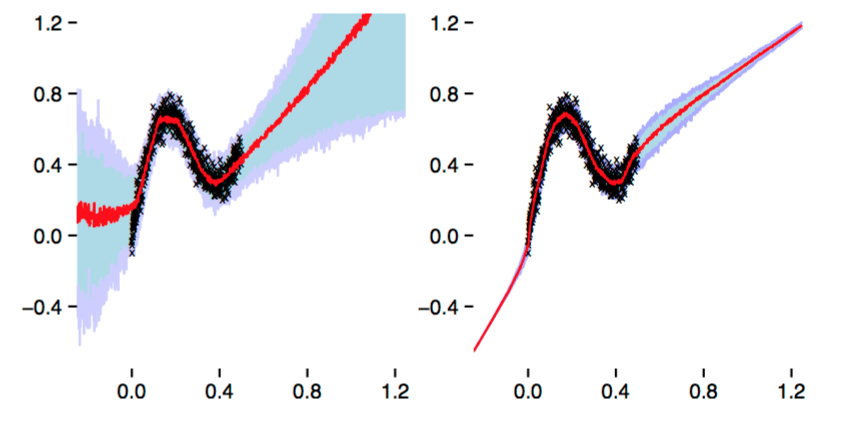
\includegraphics[width=0.9\linewidth]{05_LearningAsBayesianInference/figures/BBB_vanillaNN.png}
    	\caption{Regression of noisy data with interquatile ranges. Black crosses are training samples. Red lines are median predictions. Blue/purple region is interquartile range. \textbf{Left}: Bayes by Back- prop neural network, \textbf{Right}: standard neural network. Blundell et al., 2015} 
    	\label{fig:bbb_vanillaNN}
    \end{figure}
    
    \item \textbf{Better generalization}: Algorithm shows good results on MNIST dataset; its learning curve is comparable to that of dropout ("although each iteration of Bayes by Backprop is more expensive than dropout – around two times slower" (Blundell et al., 2015)). One of the advantages of this approach is that a good prior can be considered as additional data.
    \begin{figure}[H]
    	\centering
    	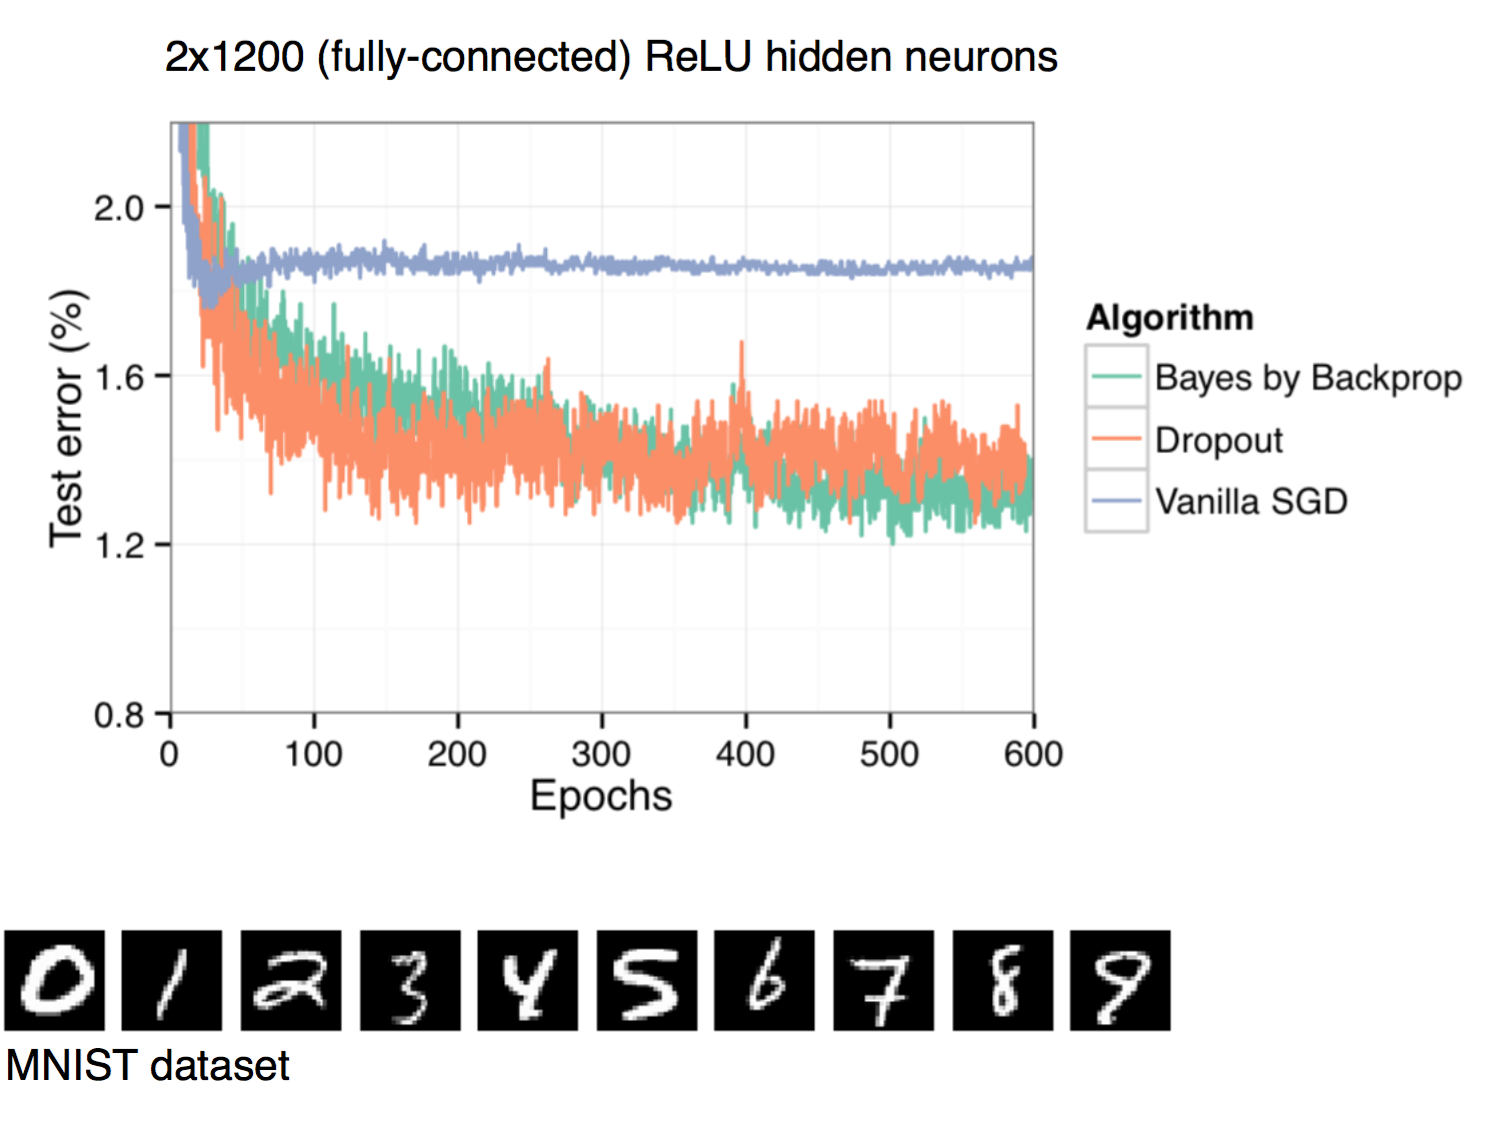
\includegraphics[width=0.9\linewidth]{05_LearningAsBayesianInference/figures/learningcurve_bbb.png}
    	\caption{Test error on MNIST as training progresses.} 
    	\label{fig:bbb_testerror}
    \end{figure}
    
    \item \textbf{Outlier detection} which is crucial for high-risk systems
    \item \textbf{Continual learning}\\
        \hl{Kirkpatrick et al., 2017, Nguyen et al., 2018}
\end{enumerate}

\subsection{Drawbacks and Weaknesses of BbB}
\hl{Discuss}
One obvious drawback is that it is computationally expensive..

\subsection{BbB and Neuroscience}
Now the question is how to interpret or think about BbB from a neuroscience perspective?

\noindent One way to think about Bayes by Backprop is to see it as a model of inference with \textbf{stochastic synapses}.

\begin{center}
% \begin{adjustbox}{width=\textwidth}
    \begin{tabular}{|p{5cm}|p{7cm}|}
    \hline
     Bayes by Backprop Algorithm & How to think about it in the brain?\\\\
     \hline
     \hline
    Independent weight sampling &  Noisy synaptic transmission. Every time the an input is propagated, the mean weight $\mu$ is corrupted by additive Gaussian noise.\\
    \hline\\
    Learning changes both the mean synaptic weight $\mu$ and the level of synaptic variability $\sigma^2$ & Can it be considered as “higher order” form of synaptic plasticity?  \\ 
    \hline\\
    Independent synapses assumption in q(w) &  Extra terms in the learning rules are local to synapses \\ 
    \hline
    \end{tabular}
% \end{adjustbox}
\end{center}

\subsubsection{Synaptic transmission in the brain}
Some key facts to note \footnote{Llera1, Sacramento and Costa. Computational roles of plastic probabilistic synapses. 2019}
\begin{itemize}
    \item Synaptic transmission is inherently stochastic, meaning that a pre-synaptic action potential may and may not trigger neurotransmitter release.
    \item There is evidence that plasticity changes the properties (modifies the mean and variance of 
    synaptic response) and number of postsynaptic receptors, as well as the presynaptic "machinery" responsible for stochastic neurotransmitter release.
    \item Probabilistic nature of synaptic transmission has been describes as a binomial process process parametrised by
        \begin{enumerate}
            \item Number of synaptic release sites N
            \item Presynaptic release probability $P_{rel}$
            \item Quantal amplitude q (proportional to the number of postsynaptic receptors)
        \end{enumerate}
    This allows us to define the statistics of synaptic responses with
    \begin{equation}
        \begin{split}
            & mean = N q P_{rel}\\
            & Var = N q^2 P_{rel} (1-P_{rel})
        \end{split}
    \end{equation}
 
    \begin{figure}[H]
    	\centering
    	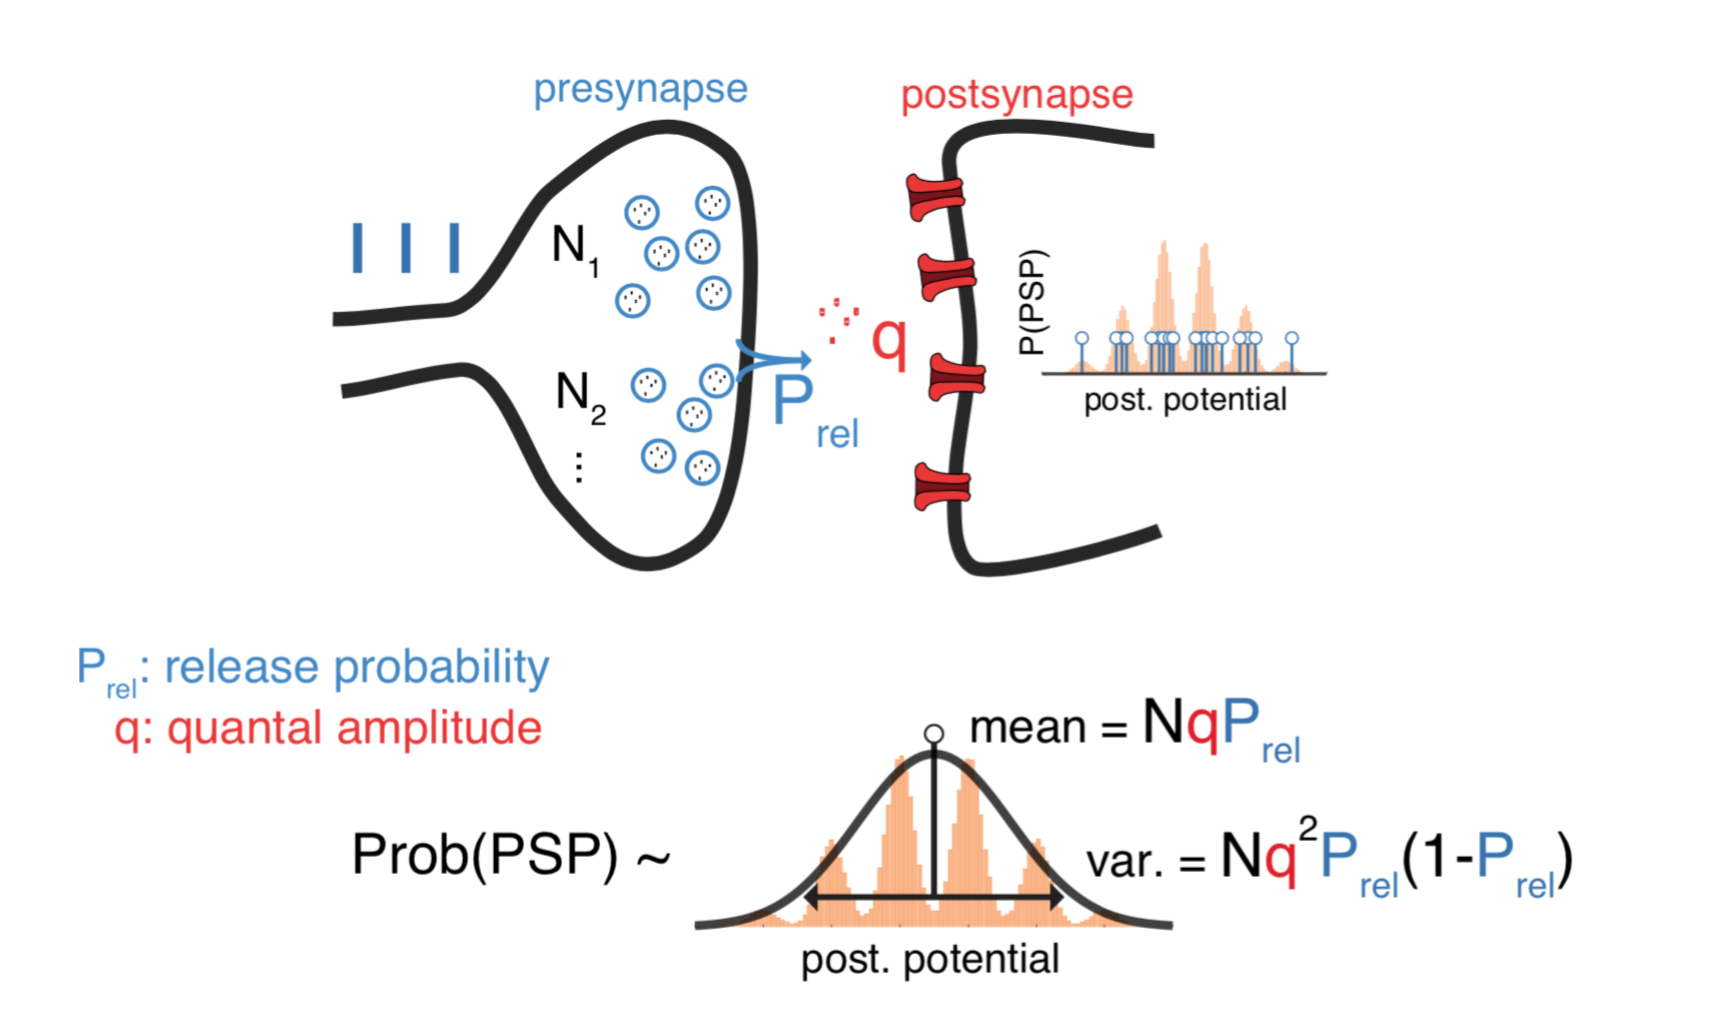
\includegraphics[width=0.9\linewidth]{05_LearningAsBayesianInference/figures/synaptic_tx_model.png}
    	\caption{"When a presynaptic spike (blue vertical line on the left) occurs a presynaptic vesicle (blue circles) may release neurotransmitters (red dots) that bind to postsynaptic receptors (red) which elicits a postsynaptic potential (PSP; PSPs of different amplitudes are represented by the small vertical blue lines)" (extracted Llera,2019)} 
    	\label{fig:synaptic_tx}
    \end{figure}
    
    \item Currently under study: what is the locus of plasticity? 
        \begin{itemize}
            \item [--] It is currently accepted that both pre- and postsynaptic physiology can be modified during long-term potentiation (LTP) and depression (LTD)
        \end{itemize}
        
     \begin{figure}[H]
    	\centering
    	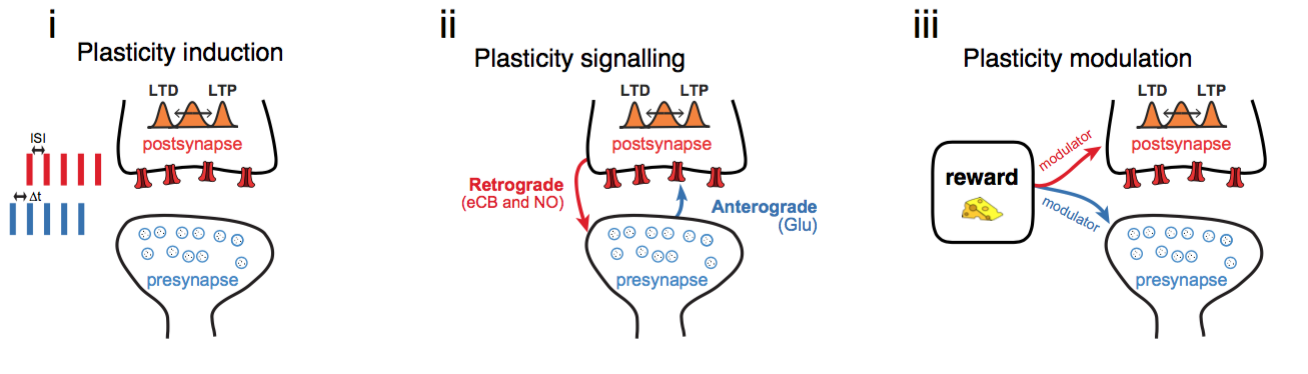
\includegraphics[width=0.9\linewidth]{05_LearningAsBayesianInference/figures/longterm_plasticity.png}
    	\caption{Long-term plasticity of probabilistic synapses. (i) Different induction protocols have been shown to trigger changes in the probability of postsynaptic responses. Schematic on the left represents pre- and postsynaptic spikes in a spike- timing-dependent plasticity protocol, which depending on the timing between pre- and postsynaptic spikes (∆t) as well as the inter-spike interval (ISI) may lead to long-term potentiation (LTP) or depression (LTD). This in turn changes not only the mean synaptic response, but also its variance. (ii) Modifications to probabilistic synapses during plasticity are known to rely on specific retrograde (e.g. endocannabinoids (eCB) and nitric oxide (NO)) and anterograde signals (glutamate (Glu)). (iii) Behavioural outcomes (e.g. reward) may rely on neuromodulation (e.g. Dopamine) to regulate plasticity at probabilistic synapses. (extracted from Llera,2019)} 
    	\label{fig:synaptic_tx}
    \end{figure}
\end{itemize}

\subsubsection{Interlude on behavioral studies}
\paragraph{Goal:} This study aim is to show how the human brain makes predictions in presence of parameter uncertainty. The question the authors ask is: Do humans take advantage of Bayesian regression?


\paragraph{Experimental Protocol:}
\begin{itemize}
    \item Participants were asked to extrapolate a parabola from 4 noisy points. They had to adjust the location of a $5^{th}$ point to match the curve.  
    \item Quadratic parameters of the parabola were generated from a prior distribution.
    \item After each trial, participants were shown the true parabola generating the dots as feedback. The idea here was to help them learn both the prior and the generative model.
    
\end{itemize}

\paragraph{Results:} 
\begin{itemize}
    \item Out of 4 different regression models, Bayesian regression (BR) model which takes full parameter uncertainty into account) best explains human behavior
    \item For large noise levels BR approaches null model (prior-based regression which replaces the posterior with the prior, i.e., it does not use the likelihood.)
\end{itemize}
 \begin{figure}[H]
    	\centering
    	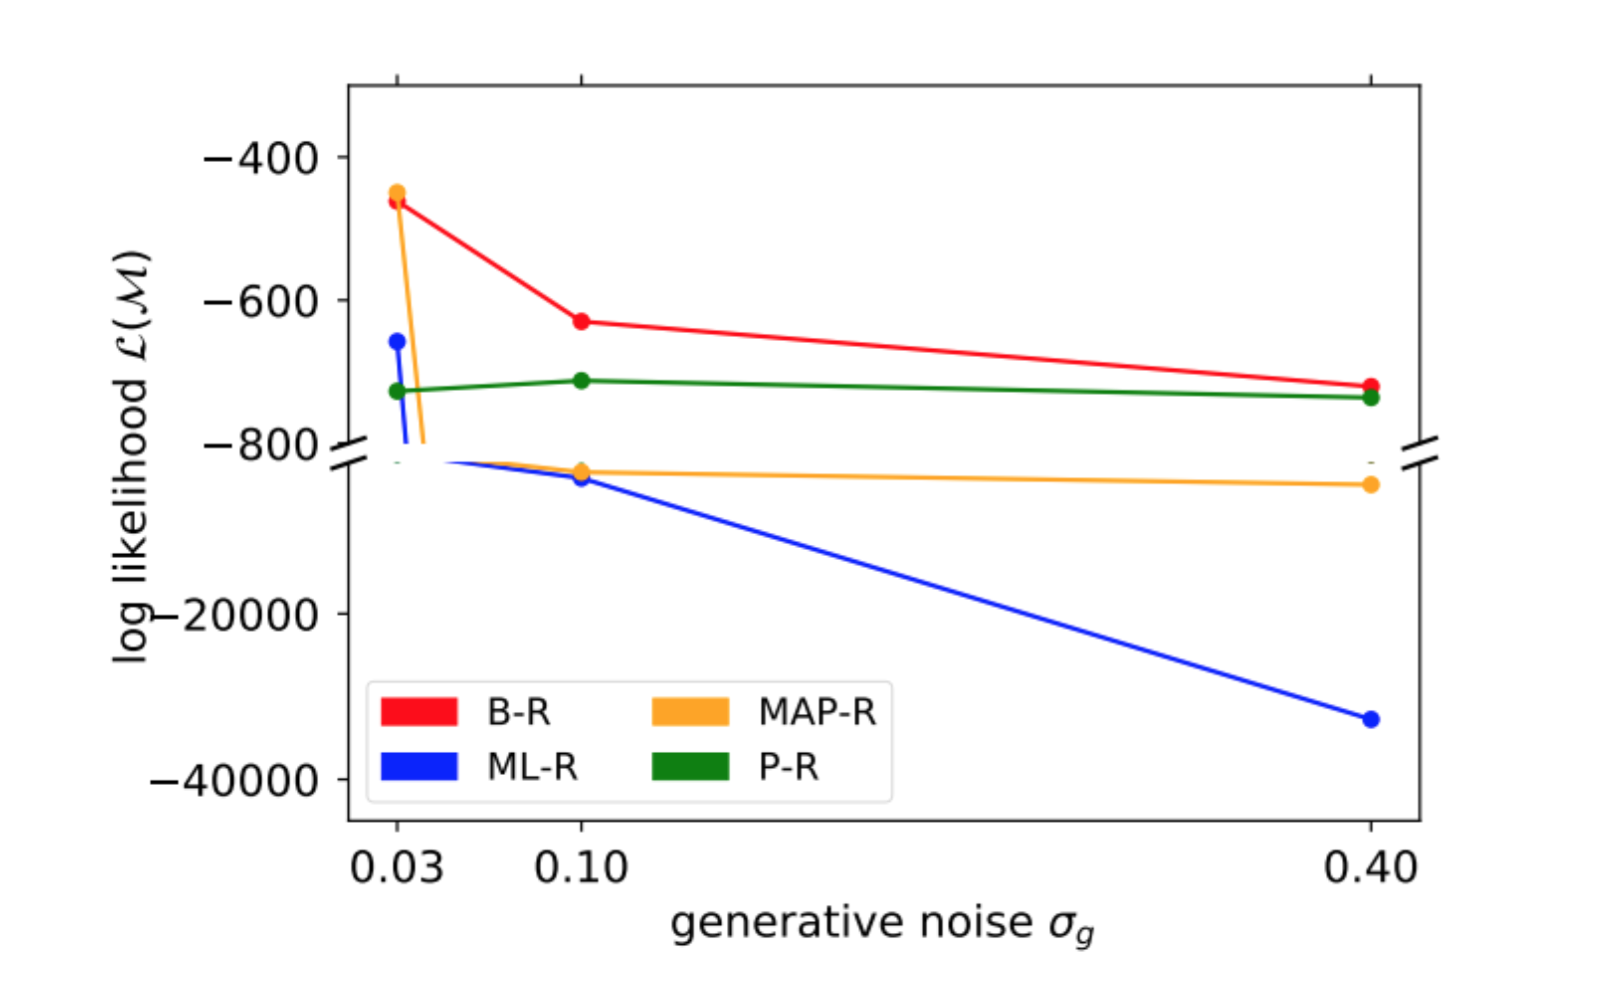
\includegraphics[width=0.9\linewidth]{05_LearningAsBayesianInference/figures/human_behavorial_exp.png}
    	\caption{Log likelihoods that the models reproduce the participant responses, i.e., the y-position adjusted by the participant averaged across participants. The higher the value, the better the model performance.\\ B-R: Bayesian Regression, ML-R: Maximum likelihood regression, MAP-R:maximum a posteriori model, P-R: prior-based regression.} 
    	\label{fig:experiment}
    \end{figure}

\end{document}
